
\subsection{Chemical Mechanisms} \label{ss:mechanisms}

{
    \renewcommand{\arraystretch}{1.3}
    \begin{table}
        \begin{center}
            \begin{tabular}{llll}
                \hline \hline
                \textbf{Chemical} & \textbf{Number of} & \textbf{Number of} & \textbf{Type of} \\ 
                \textbf{Mechanism} & \textbf{Organic Species} & \textbf{Organic Reactions} & \textbf{VOC Lumping} \\ \hline
                MCM v3.2 & $5708$ & $16349$ & No lumping \\ \hline
                MCM v3.1 & $4351$ & $12691$ & No lumping \\ \hline
                CRI v2 & $411$ & $1145$ & Lumped intermediates \\ \hline
                MOZART-4 & $69$ & $145$ & Lumped molecule \\ \hline
                RADM2 & $44$ & $103$ & Lumped molecule \\ \hline
                RACM & $58$ & $193$ & Lumped molecule \\ \hline
                RACM2 & $99$ & $315$ & Lumped molecule \\ \hline
                CBM-IV & $20$ & $45$ & Lumped structure \\ \hline
                CB05 & $37$ & $99$ & Lumped structure \\ 
                \hline \hline
            \end{tabular}
        \end{center}
        \caption{The chemical mechanisms used in the study, MCM v3.2 is the reference mechanism. References for the mechanisms are found within the main text.}
        \label{t:mechanisms}
    \end{table}
}

The chemical mechanisms used in this study are outlined in Table \ref{t:mechanisms}. 
This includes the reference mechanism (MCM v3.2) and other mechanisms that are used for both global and regional modelling. 

%MCM
The Master Chemical Mechanism (MCM) \citep{Jenkin:1997, Jenkin:2003, Saunders:2003, Bloss:2005, MCM_Site} is a near-explicit mechanism that describes the degradation of 125 primary VOCs. 
The latest version, MCM v3.2, is the reference mechanism in this study.

%CRI
The second version of the Common Representative Intermediates (CRI v2) \citep{Jenkin:2008} is a reduced chemical mechanism which describes the oxidation of the same primary VOCs as the MCM v3.1, the previous MCM version. 
VOC degradation is represented through degradation species whose \ce{O3} production reflects that of the \mbox{MCM v3.1}. 
The \mbox{CRI v2} full version (\url{http://mcm.leeds.ac.uk/CRI}) was used here.

Differences in \ce{O3} production between the CRI v2 and MCM v3.2 may be due to differences between the MCM versions rather than the reduction techniques used in the CRI v2. 
For this reason, the MCM v3.1 is also included in this study.

%MOZART
The Model for OZone and Related chemical Tracers version 4 (MOZART-4) is a global chemical transport model including its own representation of tropospheric and stratospheric chemistry \citep{Emmons:2010}. 
Methane, ethane, propane, ethene, propene, isoprene and $\alpha$-pinene are represented by non-lumped model species. 
The mechanism species BIGALK, BIGENE and TOLUENE represent all other VOC. 
The choice of mechanism species is based on the functional group of the VOC.

%RADM2
The second generation Regional Acid Deposition Model (RADM2) was developed for regional scale modelling of atmospheric chemistry \citep{Stockwell:1990}. 
Methane, ethane, ethene and isoprene are represented by explicit model species. 
All other VOCs are split into lumped model species based upon OH-reactivity and molecular weight.

%RACM
RADM2 was updated to the Regional Atmospheric Chemistry Mechanism (RACM) \citep{Stockwell:1997}. 
Updates include more explicit and mechanism species representing VOCs as well as revised rate constants and product yields. 
Aromatic, PAN and isoprene chemistry was also revised.

%RACM2
RACM2 is the most current version of the RACM mechanism \citep{Goliff:2013} with substantial updates to aromatic and ketone chemistry. 
More mechanism and explicit species representing emitted VOC are included in RACM2 leading to a more detailed mechanism than its previous versions.

%CBM4
The Carbon Bond Mechanism version four (CBM-IV) was developed for simulations of urban polluted conditions \citep{Gery:1989}. 
Ethene, formaldehyde and isoprene are the only VOCs represented by explicit species. 
All other emitted VOC are lumped according to their carbon bond types. 

Initial mixing ratios of primary VOCs were split into the appropriate representation using the method described in \citet{Hogo:1989}. 
For example, pentane has five single carbon bonds and is represented as $5$ PAR, where PAR represents carbon with only single bonds. 
An initial mixing ratio of $1,200$ pptv would be assigned as \mbox{$6,000$ ($= 1,200 \times 5$) pptv} in CBM-IV.

%CB05
The fifth version of the Carbon Bond Mechanism (CB05) \citep{Yarwood:2005} includes species representing methane, ethane and acetaldehyde. 
The chemistry schemes were revised to include peroxide formation that occurs in VOC-sensitive regions. 
The allocation of some primary VOC to mechanism species was also updated.

\subsection{Model Setup} \label{ss:model_setup}

\begin{sidewaystable}
    \begin{center}
        \begin{tabular}{lllllllll}
            \hline \hline
            \multirow{2}{*}{\textbf{NMVOC}} & \textbf{Mixing Ratio} & \textbf{MCM v3.1, v3.2} & \multirow{2}{*}{\textbf{MOZART-4}} & \multirow{2}{*}{\textbf{RADM2}} & \multirow{2}{*}{\textbf{RACM}} & \multirow{2}{*}{\textbf{RACM2}} & \multirow{2}{*}{\textbf{CBM-IV}} & \multirow{2}{*}{\textbf{CB05}}\\ & \textbf{(ppbv)} & \textbf{and CRI v2} & & & & & & \\ 
            \hline \hline \multicolumn{9}{c}{\textbf{Alkanes}}  \\ \hline
            Ethane & $6610$ & C2H6 & C2H6 & ETH & ETH & ETH & $0.4$ PAR & ETHA \\
            Propane  & $6050$ & C3H8 & C3H8 & HC3 & HC3 & HC3 & $1.5$ PAR & $1.5$ PAR \\
            Butane & $2340$ & NC4H10 & BIGALK & HC3 & HC3 & HC3 & $4$ PAR & $4$ PAR \\
            $2$-Methylpropane & $1240$ & IC4H10 & BIGALK & HC3 & HC3 & HC3 & $4$ PAR & $4$ PAR \\
            Pentane & $1200$ & NC5H12 & BIGALK & HC5 & HC5 & HC5 & $5$ PAR & $5$ PAR \\
            $2$-Methylbutane & $2790$ & IC5H12 & BIGALK & HC5 & HC5 & HC5 & $5$ PAR & $5$ PAR \\
            Hexane & $390$ & NC6H14 & BIGALK & HC5 & HC5 & HC5 & $6$ PAR & $6$ PAR \\
            Heptane & $160$ & NC7H16 &  BIGALK & HC5 & HC5 & HC5 & $7$ PAR & $7$ PAR \\
            Octane & $80$ & NC8H18 & BIGALK & HC8 & HC8 & HC8 & $8$ PAR & $8$ PAR \\ \hline 
            \multicolumn{9}{c}{\textbf{Alkenes}} \\ \hline
            Ethene & $2430$ & C2H4 & C2H4 & OL2 & ETE & ETE & ETH & ETH \\
            \multirow{2}{*}{Propene} & \multirow{2}{*}{$490$} & \multirow{2}{*}{C3H6} & \multirow{2}{*}{C3H6} & \multirow{2}{*}{OLT} & \multirow{2}{*}{OLT} & \multirow{2}{*}{OLT} & OLE + & OLE + \\ & & & & & & & \hspace{3mm}PAR & \hspace{3mm}PAR \\
            \multirow{2}{*}{Butene} & \multirow{2}{*}{$65$} & \multirow{2}{*}{BUT1ENE} & \multirow{2}{*}{BIGENE} & \multirow{2}{*}{OLT} & \multirow{2}{*}{OLT} & \multirow{2}{*}{OLT} & OLE + & OLE + \\ & & & & & & & \hspace{3mm}$2$ PAR & \hspace{3mm}$2$ PAR \\
            \multirow{2}{*}{$2$-Methylpropene} & \multirow{2}{*}{$130$} & \multirow{2}{*}{MEPROPENE} & \multirow{2}{*}{BIGENE} & \multirow{2}{*}{OLI} & \multirow{2}{*}{OLI} & \multirow{2}{*}{OLI} & \multirow{2}{*}{$2$ ALD2} & FORM + \\ & & & & & & & & \hspace{3mm}$3$ PAR \\
            Isoprene & $270$ & C5H8 & ISOP & ISO & ISO & ISO & ISOP & ISOP \\ \hline
            \multicolumn{9}{c}{\textbf{Aromatics}} \\ \hline 
            Benzene & $480$ & BENZENE & TOLUENE & TOL & TOL & BEN & PAR & PAR \\
            Toluene & $1380$ & TOLUENE & TOLUENE & TOL & TOL & TOL & TOL & TOL \\
            m-Xylene & $410$ & MXYL & TOLUENE & XYL & XYL & XYM & XYL & XYL \\
            p-Xylene & $210$ & PXYL & TOLUENE & XYL & XYL & XYP & XYL & XYL \\
            o-Xylene & $200$ & OXYL & TOLUENE & XYL & XYL & XYO & XYL & XYL \\
            \multirow{2}{*}{Ethylbenzene} & \multirow{2}{*}{$210$} & \multirow{2}{*}{EBENZ} & \multirow{2}{*}{TOLUENE} & \multirow{2}{*}{TOL} & \multirow{2}{*}{TOL} & \multirow{2}{*}{TOL} & TOL + & TOL + \\ & & & & & & & \hspace{3mm}PAR & \hspace{3mm}PAR \\ \hline \hline
        \end{tabular}
    \end{center}
    \caption{Typical NMVOCs present in Los Angeles and their respective mixing ratios \citep{Baker:2008} as well as their representation in each chemical mechanism. The representation of the VOCs in each mechanism is based upon the recommendations of the respective literature.}
    \label{t:initial_conditions}
\end{sidewaystable}

%general info
The modelling approach and set-up followed that of the original TOPP study of \citet{Butler:2011}.
A summary is provided, further details are found in the supplement to this paper and in \citet{Butler:2011}. 
The radical and \ce{NO_x} amounts were balanced at each time step by emitting the amount of NO equalling the total radical source minus the total \ce{NO_x} source.
The NO emission amounts were determined separately for each model run ensuring conditions of maximum \ce{O3} production for each mechanism.

%initial conditions
The NMVOC and their initial mixing ratios are those of Los Angeles taken from \citet{Baker:2008}. 
The initial NMVOC mixing ratios were held constant until midday of the first day and then left to react freely. 
Methane (\ce{CH4}) was held fixed at \mbox{$1.8$ ppmv}. 
Carbon monoxide (CO) and \ce{O3} were initialised at \mbox{$200$ ppbv} and \mbox{$40$ ppbv} respectively and then allowed to evolve freely.

Table \ref{t:initial_conditions} outlines the NMVOC used in the study, their initial mixing ratios and representation in the different mechanisms.
The mechanism assignment of each NMVOC followed the recommendations for each mechanism.
Initial mixing ratios were weighted by carbon number of the mechanism species when lumping NMVOC into mechanism species. 
This ensured the initial amount of reactive carbon was constant between model runs.

\subsubsection{Mechanism Implementation} %implementation of mechanisms for the runs

The MECCA boxmodel \citep{Sander:2005} is based upon the Kinetic Pre-Processor (KPP) \citep{Damian:2002} and was used as described in \citet{Butler:2011}. 
Hence, all chemical mechanisms were adapted into the modularised KPP format.

The MCM v3.2 inorganic chemistry reactions were used in each model run to focus on the organic NMVOC degradation chemistry.
Inorganic gas-phase chemistry is relatively well-known and any differences are typically due to inconsistencies between IUPAC and JPL reaction rate constants \citep{Emmerson:2009}.

Some mechanisms include reactions which are important only in the stratosphere or free troposphere. 
Such reactions were not included as this study is concerned with processes below the planetary boundary layer. 
For example, PAN photolysis was removed from MOZART-4, RACM2 and CB05 as it is only important in the free troposphere \citep{Harwood:2003}.  

The MCM v3.2 approach to photolysis, dry deposition and peroxy radical -- peroxy radical reactions was used for each mechanism. 
The supplement to this article contains a detailed description of this implementation.

\subsection{Tagged Ozone Production Potential (TOPP)}
This section summarises the tagging methodology described in \citet{Butler:2011} which should be consulted for more details.

\subsubsection[Tagging Approach and Application to Ox Family]{Tagging Approach and Application to \ce{O_x} Family} \label{ss:tagging} %tagging of mechanisms

Tagging follows the degradation of all NMVOCs in Table \ref{t:initial_conditions} through all possible degradation pathways. 
The chemical mechanisms were re-written with every organic degradation product labelled with the name of the emitted NMVOC. 
Thus, each NMVOC has its own set of degradation reactions \citep{Butler:2011}. 

\begin{figure}
    \begin{center}
        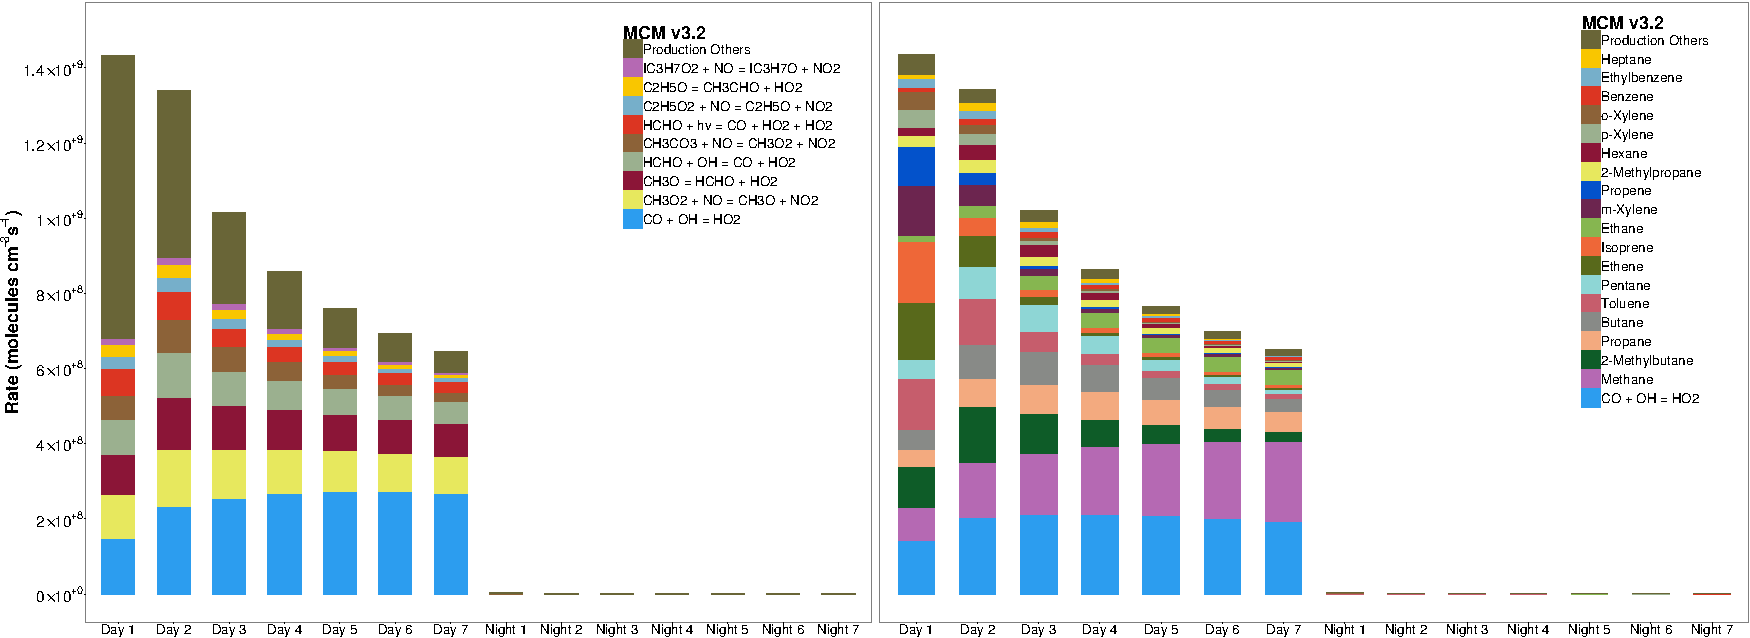
\includegraphics[width=\textwidth]{img/MCMv3_2_Ox_production_budgets}
        \caption{The \ce{O_x} production budgets using the MCM v3.2 (a) without tagging and \mbox{(b) with} tagging, where \ce{O_x} production is attributed to the emitted VOCs.}
        \label{f:Ox_budget}
    \end{center}
\end{figure} 

The tagging approach allows allocation of production and consumption budgets to emitted NMVOCs. 
Without tagging, the individual reactions responsible for \ce{O_x} production can be determined but not the NMVOC source of the organic reactants. 
The NMVOC source can be determined by examination of the tagged species, as illustrated in \mbox{Figure \ref{f:Ox_budget}}.

\subsubsection{Tagged Ozone Production Potential (TOPP) Definition} %final definition of TOPP

The TOPP is the ratio of \ce{O_x} molecules produced per molecule of emitted VOC.  
Daily TOPP values are calculated by determining the total daily contribution to \ce{O_x} production from a VOC and then normalising by its total emissions on the first day of the model run. 
The \ce{O_x} production of each VOC is determined by means of the tags as described in \mbox{Section \ref{ss:tagging}}. 
